\documentclass[1p]{elsarticle_modified}
%\bibliographystyle{elsarticle-num}

%\usepackage[colorlinks]{hyperref}
%\usepackage{abbrmath_seonhwa} %\Abb, \Ascr, \Acal ,\Abf, \Afrak
\usepackage{amsfonts}
\usepackage{amssymb}
\usepackage{amsmath}
\usepackage{amsthm}
\usepackage{scalefnt}
\usepackage{amsbsy}
\usepackage{kotex}
\usepackage{caption}
\usepackage{subfig}
\usepackage{color}
\usepackage{graphicx}
\usepackage{xcolor} %% white, black, red, green, blue, cyan, magenta, yellow
\usepackage{float}
\usepackage{setspace}
\usepackage{hyperref}

\usepackage{tikz}
\usetikzlibrary{arrows}

\usepackage{multirow}
\usepackage{array} % fixed length table
\usepackage{hhline}

%%%%%%%%%%%%%%%%%%%%%
\makeatletter
\renewcommand*\env@matrix[1][\arraystretch]{%
	\edef\arraystretch{#1}%
	\hskip -\arraycolsep
	\let\@ifnextchar\new@ifnextchar
	\array{*\c@MaxMatrixCols c}}
\makeatother %https://tex.stackexchange.com/questions/14071/how-can-i-increase-the-line-spacing-in-a-matrix
%%%%%%%%%%%%%%%

\usepackage[normalem]{ulem}

\newcommand{\msout}[1]{\ifmmode\text{\sout{\ensuremath{#1}}}\else\sout{#1}\fi}
%SOURCE: \msout is \stkout macro in https://tex.stackexchange.com/questions/20609/strikeout-in-math-mode

\newcommand{\cancel}[1]{
	\ifmmode
	{\color{red}\msout{#1}}
	\else
	{\color{red}\sout{#1}}
	\fi
}

\newcommand{\add}[1]{
	{\color{blue}\uwave{#1}}
}

\newcommand{\replace}[2]{
	\ifmmode
	{\color{red}\msout{#1}}{\color{blue}\uwave{#2}}
	\else
	{\color{red}\sout{#1}}{\color{blue}\uwave{#2}}
	\fi
}

\newcommand{\Sol}{\mathcal{S}} %segment
\newcommand{\D}{D} %diagram
\newcommand{\A}{\mathcal{A}} %arc


%%%%%%%%%%%%%%%%%%%%%%%%%%%%%5 test

\def\sl{\operatorname{\textup{SL}}(2,\Cbb)}
\def\psl{\operatorname{\textup{PSL}}(2,\Cbb)}
\def\quan{\mkern 1mu \triangleright \mkern 1mu}

\theoremstyle{definition}
\newtheorem{thm}{Theorem}[section]
\newtheorem{prop}[thm]{Proposition}
\newtheorem{lem}[thm]{Lemma}
\newtheorem{ques}[thm]{Question}
\newtheorem{cor}[thm]{Corollary}
\newtheorem{defn}[thm]{Definition}
\newtheorem{exam}[thm]{Example}
\newtheorem{rmk}[thm]{Remark}
\newtheorem{alg}[thm]{Algorithm}

\newcommand{\I}{\sqrt{-1}}
\begin{document}

%\begin{frontmatter}
%
%\title{Boundary parabolic representations of knots up to 8 crossings}
%
%%% Group authors per affiliation:
%\author{Yunhi Cho} 
%\address{Department of Mathematics, University of Seoul, Seoul, Korea}
%\ead{yhcho@uos.ac.kr}
%
%
%\author{Seonhwa Kim} %\fnref{s_kim}}
%\address{Center for Geometry and Physics, Institute for Basic Science, Pohang, 37673, Korea}
%\ead{ryeona17@ibs.re.kr}
%
%\author{Hyuk Kim}
%\address{Department of Mathematical Sciences, Seoul National University, Seoul 08826, Korea}
%\ead{hyukkim@snu.ac.kr}
%
%\author{Seokbeom Yoon}
%\address{Department of Mathematical Sciences, Seoul National University, Seoul, 08826,  Korea}
%\ead{sbyoon15@snu.ac.kr}
%
%\begin{abstract}
%We find all boundary parabolic representation of knots up to 8 crossings.
%
%\end{abstract}
%\begin{keyword}
%    \MSC[2010] 57M25 
%\end{keyword}
%
%\end{frontmatter}

%\linenumbers
%\tableofcontents
%
\newcommand\colored[1]{\textcolor{white}{\rule[-0.35ex]{0.8em}{1.4ex}}\kern-0.8em\color{red} #1}%
%\newcommand\colored[1]{\textcolor{white}{ #1}\kern-2.17ex	\textcolor{white}{ #1}\kern-1.81ex	\textcolor{white}{ #1}\kern-2.15ex\color{red}#1	}

{\Large $\underline{12a_{0062}~(K12a_{0062})}$}

\setlength{\tabcolsep}{10pt}
\renewcommand{\arraystretch}{1.6}
\vspace{1cm}\begin{tabular}{m{100pt}>{\centering\arraybackslash}m{274pt}}
\multirow{5}{120pt}{
	\centering
	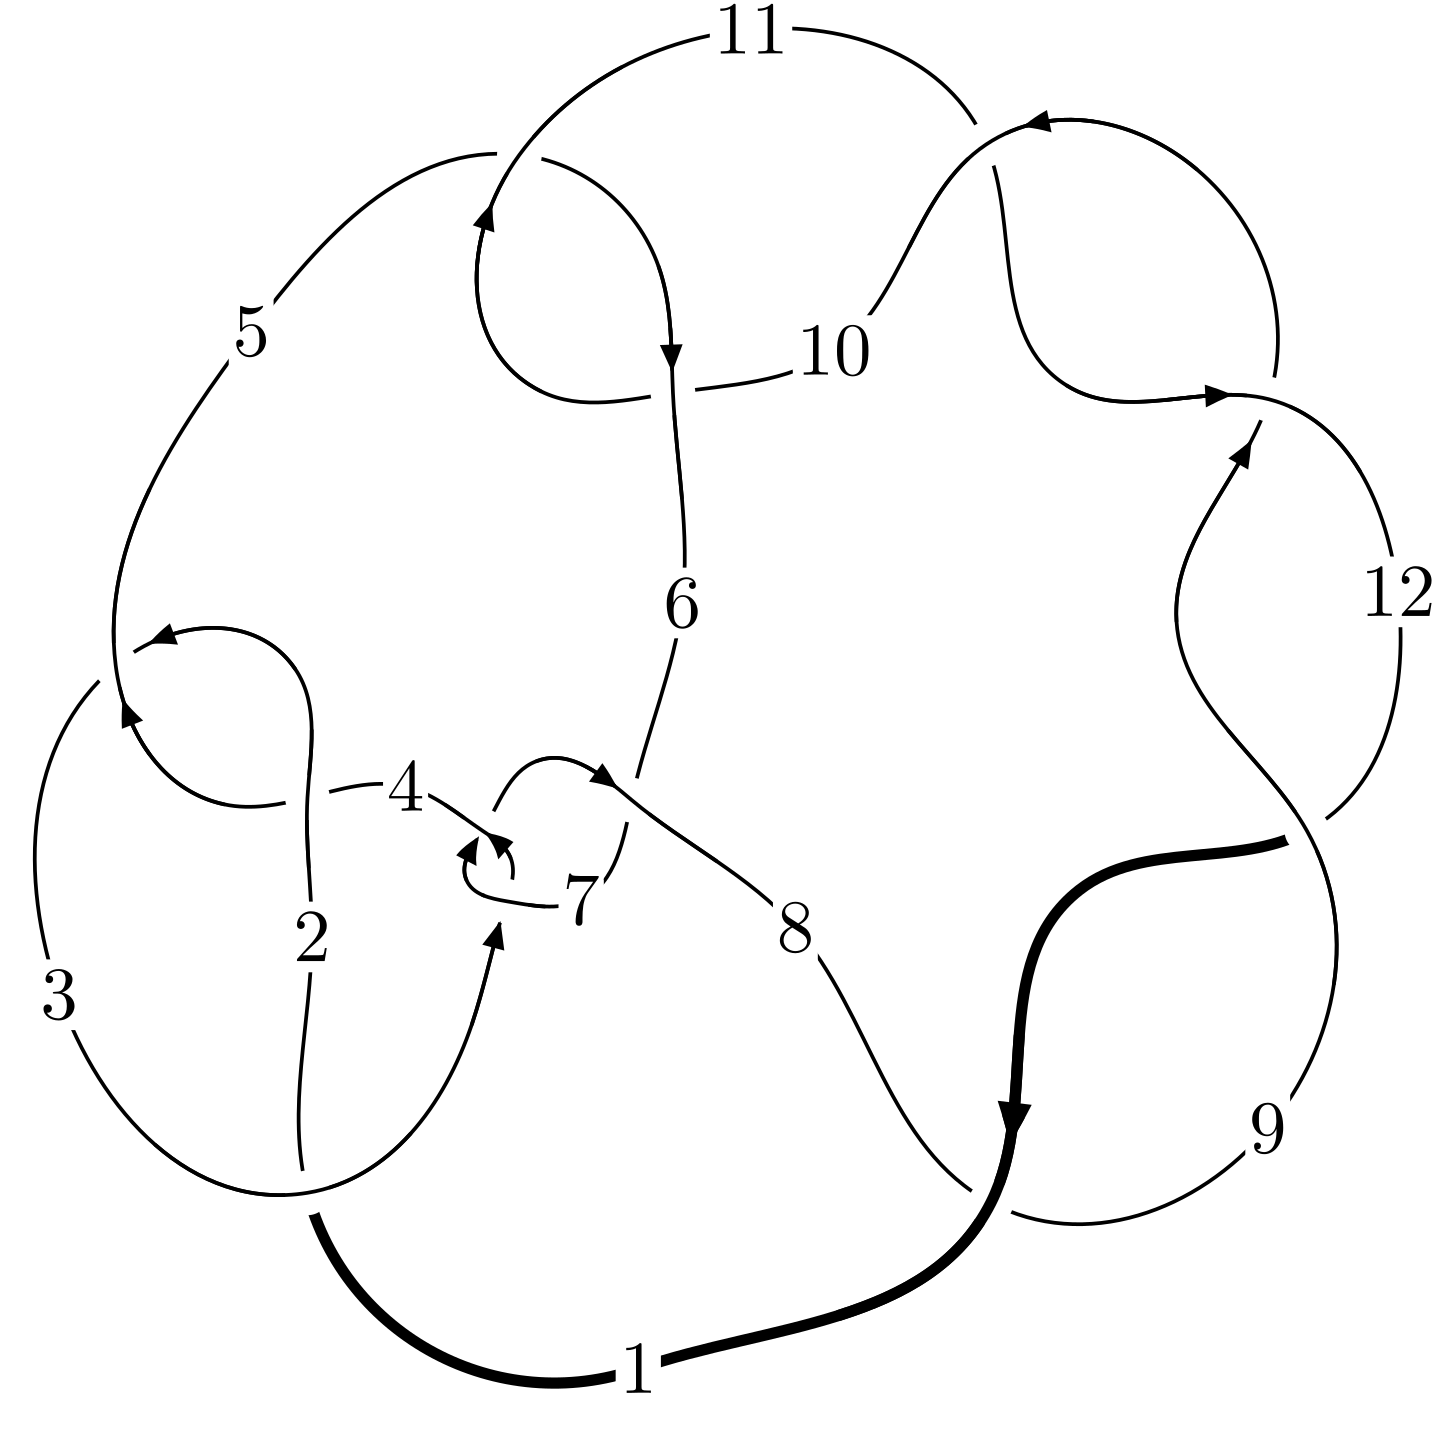
\includegraphics[width=112pt]{../../../GIT/diagram.site/Diagrams/png/863_12a_0062.png}\\
\ \ \ A knot diagram\footnotemark}&
\allowdisplaybreaks
\textbf{Linearized knot diagam} \\
\cline{2-2}
 &
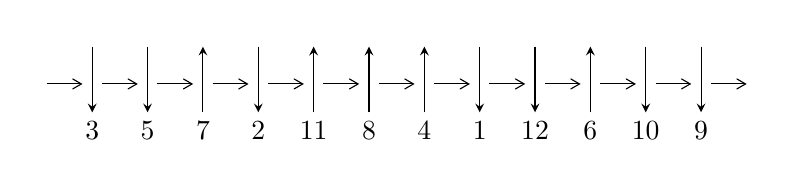
\begin{tikzpicture}[x=20pt, y=17pt]
	% nodes
	\node (C0) at (0, 0) {};
	\node (C1) at (1, 0) {};
	\node (C1U) at (1, +1) {};
	\node (C1D) at (1, -1) {3};

	\node (C2) at (2, 0) {};
	\node (C2U) at (2, +1) {};
	\node (C2D) at (2, -1) {5};

	\node (C3) at (3, 0) {};
	\node (C3U) at (3, +1) {};
	\node (C3D) at (3, -1) {7};

	\node (C4) at (4, 0) {};
	\node (C4U) at (4, +1) {};
	\node (C4D) at (4, -1) {2};

	\node (C5) at (5, 0) {};
	\node (C5U) at (5, +1) {};
	\node (C5D) at (5, -1) {11};

	\node (C6) at (6, 0) {};
	\node (C6U) at (6, +1) {};
	\node (C6D) at (6, -1) {8};

	\node (C7) at (7, 0) {};
	\node (C7U) at (7, +1) {};
	\node (C7D) at (7, -1) {4};

	\node (C8) at (8, 0) {};
	\node (C8U) at (8, +1) {};
	\node (C8D) at (8, -1) {1};

	\node (C9) at (9, 0) {};
	\node (C9U) at (9, +1) {};
	\node (C9D) at (9, -1) {12};

	\node (C10) at (10, 0) {};
	\node (C10U) at (10, +1) {};
	\node (C10D) at (10, -1) {6};

	\node (C11) at (11, 0) {};
	\node (C11U) at (11, +1) {};
	\node (C11D) at (11, -1) {10};

	\node (C12) at (12, 0) {};
	\node (C12U) at (12, +1) {};
	\node (C12D) at (12, -1) {9};
	\node (C13) at (13, 0) {};

	% arrows
	\draw[->,>={angle 60}]
	(C0) edge (C1) (C1) edge (C2) (C2) edge (C3) (C3) edge (C4) (C4) edge (C5) (C5) edge (C6) (C6) edge (C7) (C7) edge (C8) (C8) edge (C9) (C9) edge (C10) (C10) edge (C11) (C11) edge (C12) (C12) edge (C13) ;	\draw[->,>=stealth]
	(C1U) edge (C1D) (C2U) edge (C2D) (C3D) edge (C3U) (C4U) edge (C4D) (C5D) edge (C5U) (C6D) edge (C6U) (C7D) edge (C7U) (C8U) edge (C8D) (C9U) edge (C9D) (C10D) edge (C10U) (C11U) edge (C11D) (C12U) edge (C12D) ;
	\end{tikzpicture} \\
\hhline{~~} \\& 
\textbf{Solving Sequence} \\ \cline{2-2} 
 &
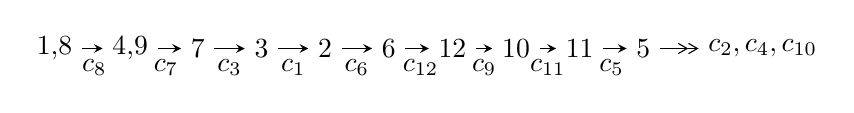
\begin{tikzpicture}[x=23pt, y=7pt]
	% node
	\node (A0) at (-1/8, 0) {1,8};
	\node (A1) at (17/16, 0) {4,9};
	\node (A2) at (17/8, 0) {7};
	\node (A3) at (25/8, 0) {3};
	\node (A4) at (33/8, 0) {2};
	\node (A5) at (41/8, 0) {6};
	\node (A6) at (49/8, 0) {12};
	\node (A7) at (57/8, 0) {10};
	\node (A8) at (65/8, 0) {11};
	\node (A9) at (73/8, 0) {5};
	\node (C1) at (1/2, -1) {$c_{8}$};
	\node (C2) at (13/8, -1) {$c_{7}$};
	\node (C3) at (21/8, -1) {$c_{3}$};
	\node (C4) at (29/8, -1) {$c_{1}$};
	\node (C5) at (37/8, -1) {$c_{6}$};
	\node (C6) at (45/8, -1) {$c_{12}$};
	\node (C7) at (53/8, -1) {$c_{9}$};
	\node (C8) at (61/8, -1) {$c_{11}$};
	\node (C9) at (69/8, -1) {$c_{5}$};
	\node (A10) at (11, 0) {$c_{2},c_{4},c_{10}$};

	% edge
	\draw[->,>=stealth]	
	(A0) edge (A1) (A1) edge (A2) (A2) edge (A3) (A3) edge (A4) (A4) edge (A5) (A5) edge (A6) (A6) edge (A7) (A7) edge (A8) (A8) edge (A9) ;
	\draw[->>,>={angle 60}]	
	(A9) edge (A10);
\end{tikzpicture} \\ 

\end{tabular} \\

\footnotetext{
The image of knot diagram is generated by the software ``\textbf{Draw programme}" developed by Andrew Bartholomew(\url{http://www.layer8.co.uk/maths/draw/index.htm\#Running-draw}), where we modified some parts for our purpose(\url{https://github.com/CATsTAILs/LinksPainter}).
}\phantom \\ \newline 
\centering \textbf{Ideals for irreducible components\footnotemark of $X_{\text{par}}$} 
 
\begin{align*}
I^u_{1}&=\langle 
4.34077\times10^{20} u^{67}-5.64426\times10^{21} u^{66}+\cdots+2.17039\times10^{21} b-1.25825\times10^{18},\\
\phantom{I^u_{1}}&\phantom{= \langle  }9.54970\times10^{20} u^{67}-1.50190\times10^{22} u^{66}+\cdots+2.17039\times10^{21} a-1.96214\times10^{22},\;u^{68}-14 u^{67}+\cdots-10 u+1\rangle \\
I^u_{2}&=\langle 
b,\;- u^3+u^2+a-3 u+2,\;u^4- u^3+3 u^2-2 u+1\rangle \\
\\
\end{align*}
\raggedright * 2 irreducible components of $\dim_{\mathbb{C}}=0$, with total 72 representations.\\
\footnotetext{All coefficients of polynomials are rational numbers. But the coefficients are sometimes approximated in decimal forms when there is not enough margin.}
\newpage
\renewcommand{\arraystretch}{1}
\centering \section*{I. $I^u_{1}= \langle 4.34\times10^{20} u^{67}-5.64\times10^{21} u^{66}+\cdots+2.17\times10^{21} b-1.26\times10^{18},\;9.55\times10^{20} u^{67}-1.50\times10^{22} u^{66}+\cdots+2.17\times10^{21} a-1.96\times10^{22},\;u^{68}-14 u^{67}+\cdots-10 u+1 \rangle$}
\flushleft \textbf{(i) Arc colorings}\\
\begin{tabular}{m{7pt} m{180pt} m{7pt} m{180pt} }
\flushright $a_{1}=$&$\begin{pmatrix}0\\u\end{pmatrix}$ \\
\flushright $a_{8}=$&$\begin{pmatrix}1\\0\end{pmatrix}$ \\
\flushright $a_{4}=$&$\begin{pmatrix}-0.440000 u^{67}+6.91995 u^{66}+\cdots-51.0249 u+9.04053\\-0.200000 u^{67}+2.60058 u^{66}+\cdots-4.04580 u+0.000579734\end{pmatrix}$ \\
\flushright $a_{9}=$&$\begin{pmatrix}1\\u^2\end{pmatrix}$ \\
\flushright $a_{7}=$&$\begin{pmatrix}-0.00405814 u^{67}-0.343186 u^{66}+\cdots-4.75480 u-1.28000\\0.599983 u^{67}-8.39976 u^{66}+\cdots+5.88404 u-0.600000\end{pmatrix}$ \\
\flushright $a_{3}=$&$\begin{pmatrix}-1.04000 u^{67}+14.7200 u^{66}+\cdots-67.3194 u+10.4464\\-0.200000 u^{67}+2.60638 u^{66}+\cdots-5.50377 u+0.00637708\end{pmatrix}$ \\
\flushright $a_{2}=$&$\begin{pmatrix}0.240000 u^{67}-4.32004 u^{66}+\cdots+46.9162 u-9.67830\\0.400000 u^{67}-5.19826 u^{66}+\cdots+5.86261 u+0.00173920\end{pmatrix}$ \\
\flushright $a_{6}=$&$\begin{pmatrix}-0.604041 u^{67}+8.05658 u^{66}+\cdots-10.6388 u-0.680000\\0.599983 u^{67}-8.39976 u^{66}+\cdots+5.88404 u-0.600000\end{pmatrix}$ \\
\flushright $a_{12}=$&$\begin{pmatrix}u\\u^3+u\end{pmatrix}$ \\
\flushright $a_{10}=$&$\begin{pmatrix}u^2+1\\u^4+2 u^2\end{pmatrix}$ \\
\flushright $a_{11}=$&$\begin{pmatrix}u^3+2 u\\u^5+3 u^3+u\end{pmatrix}$ \\
\flushright $a_{5}=$&$\begin{pmatrix}-0.600000 u^{67}+7.80002 u^{66}+\cdots-15.7984 u+0.115959\\0.400000 u^{67}-5.20406 u^{66}+\cdots+1.32058 u-0.00405814\end{pmatrix}$\\&\end{tabular}
\flushleft \textbf{(ii) Obstruction class $= -1$}\\~\\
\flushleft \textbf{(iii) Cusp Shapes $= -\frac{3420526093780033582661}{1085192982908851054063} u^{67}+\frac{48060996190185886286483}{1085192982908851054063} u^{66}+\cdots-\frac{55112703006359386129501}{1085192982908851054063} u+\frac{338580210667561528866}{1085192982908851054063}$}\\~\\
\newpage\renewcommand{\arraystretch}{1}
\flushleft \textbf{(iv) u-Polynomials at the component}\newline \\
\begin{tabular}{m{50pt}|m{274pt}}
Crossings & \hspace{64pt}u-Polynomials at each crossing \\
\hline $$\begin{aligned}c_{1}\end{aligned}$$&$\begin{aligned}
&u^{68}+35 u^{67}+\cdots+4 u+1
\end{aligned}$\\
\hline $$\begin{aligned}c_{2},c_{4}\end{aligned}$$&$\begin{aligned}
&u^{68}-5 u^{67}+\cdots-4 u+1
\end{aligned}$\\
\hline $$\begin{aligned}c_{3},c_{7}\end{aligned}$$&$\begin{aligned}
&u^{68}- u^{67}+\cdots+56 u+16
\end{aligned}$\\
\hline $$\begin{aligned}c_{5},c_{10}\end{aligned}$$&$\begin{aligned}
&u^{68}-2 u^{67}+\cdots-2 u+1
\end{aligned}$\\
\hline $$\begin{aligned}c_{6}\end{aligned}$$&$\begin{aligned}
&u^{68}-27 u^{67}+\cdots-3136 u+256
\end{aligned}$\\
\hline $$\begin{aligned}c_{8},c_{9},c_{11}\\c_{12}\end{aligned}$$&$\begin{aligned}
&u^{68}+14 u^{67}+\cdots+10 u+1
\end{aligned}$\\
\hline
\end{tabular}\\~\\
\newpage\renewcommand{\arraystretch}{1}
\flushleft \textbf{(v) Riley Polynomials at the component}\newline \\
\begin{tabular}{m{50pt}|m{274pt}}
Crossings & \hspace{64pt}Riley Polynomials at each crossing \\
\hline $$\begin{aligned}c_{1}\end{aligned}$$&$\begin{aligned}
&y^{68}+y^{67}+\cdots+28 y+1
\end{aligned}$\\
\hline $$\begin{aligned}c_{2},c_{4}\end{aligned}$$&$\begin{aligned}
&y^{68}-35 y^{67}+\cdots-4 y+1
\end{aligned}$\\
\hline $$\begin{aligned}c_{3},c_{7}\end{aligned}$$&$\begin{aligned}
&y^{68}-27 y^{67}+\cdots-3136 y+256
\end{aligned}$\\
\hline $$\begin{aligned}c_{5},c_{10}\end{aligned}$$&$\begin{aligned}
&y^{68}+14 y^{67}+\cdots+10 y+1
\end{aligned}$\\
\hline $$\begin{aligned}c_{6}\end{aligned}$$&$\begin{aligned}
&y^{68}+21 y^{67}+\cdots+1159168 y+65536
\end{aligned}$\\
\hline $$\begin{aligned}c_{8},c_{9},c_{11}\\c_{12}\end{aligned}$$&$\begin{aligned}
&y^{68}+82 y^{67}+\cdots+58 y+1
\end{aligned}$\\
\hline
\end{tabular}\\~\\
\newpage\flushleft \textbf{(vi) Complex Volumes and Cusp Shapes}
$$\begin{array}{c|c|c}  
\text{Solutions to }I^u_{1}& \I (\text{vol} + \sqrt{-1}CS) & \text{Cusp shape}\\
 \hline 
\begin{aligned}
u &= \phantom{-}0.702330 + 0.719314 I \\
a &= \phantom{-}0.952126 + 0.378495 I \\
b &= \phantom{-}0.903771 + 0.568632 I\end{aligned}
 & -2.49105 + 1.44096 I & \phantom{-0.000000 } 0 \\ \hline\begin{aligned}
u &= \phantom{-}0.702330 - 0.719314 I \\
a &= \phantom{-}0.952126 - 0.378495 I \\
b &= \phantom{-}0.903771 - 0.568632 I\end{aligned}
 & -2.49105 - 1.44096 I & \phantom{-0.000000 } 0 \\ \hline\begin{aligned}
u &= \phantom{-}0.544234 + 0.823097 I \\
a &= -0.90860 - 1.80587 I \\
b &= \phantom{-}0.787095 - 0.580214 I\end{aligned}
 & -2.86875 - 3.13470 I & \phantom{-0.000000 } 0 \\ \hline\begin{aligned}
u &= \phantom{-}0.544234 - 0.823097 I \\
a &= -0.90860 + 1.80587 I \\
b &= \phantom{-}0.787095 + 0.580214 I\end{aligned}
 & -2.86875 + 3.13470 I & \phantom{-0.000000 } 0 \\ \hline\begin{aligned}
u &= \phantom{-}0.554678 + 0.885053 I \\
a &= \phantom{-}0.646033 + 0.891159 I \\
b &= \phantom{-}0.597107 + 0.903347 I\end{aligned}
 & -2.45632 - 5.69189 I & \phantom{-0.000000 } 0 \\ \hline\begin{aligned}
u &= \phantom{-}0.554678 - 0.885053 I \\
a &= \phantom{-}0.646033 - 0.891159 I \\
b &= \phantom{-}0.597107 - 0.903347 I\end{aligned}
 & -2.45632 + 5.69189 I & \phantom{-0.000000 } 0 \\ \hline\begin{aligned}
u &= \phantom{-}0.044041 + 0.938846 I \\
a &= -0.528628 + 0.575298 I \\
b &= \phantom{-}1.110590 + 0.020786 I\end{aligned}
 & \phantom{-}4.84823 - 0.01751 I & \phantom{-0.000000 } 0 \\ \hline\begin{aligned}
u &= \phantom{-}0.044041 - 0.938846 I \\
a &= -0.528628 - 0.575298 I \\
b &= \phantom{-}1.110590 - 0.020786 I\end{aligned}
 & \phantom{-}4.84823 + 0.01751 I & \phantom{-0.000000 } 0 \\ \hline\begin{aligned}
u &= \phantom{-}0.230283 + 1.041890 I \\
a &= \phantom{-}0.383940 + 0.200681 I \\
b &= -1.096910 + 0.163946 I\end{aligned}
 & \phantom{-}4.52428 - 4.84320 I & \phantom{-0.000000 } 0 \\ \hline\begin{aligned}
u &= \phantom{-}0.230283 - 1.041890 I \\
a &= \phantom{-}0.383940 - 0.200681 I \\
b &= -1.096910 - 0.163946 I\end{aligned}
 & \phantom{-}4.52428 + 4.84320 I & \phantom{-0.000000 } 0\\
 \hline 
 \end{array}$$\newpage$$\begin{array}{c|c|c}  
\text{Solutions to }I^u_{1}& \I (\text{vol} + \sqrt{-1}CS) & \text{Cusp shape}\\
 \hline 
\begin{aligned}
u &= \phantom{-}0.886908 + 0.130997 I \\
a &= \phantom{-}0.83919 - 1.48134 I \\
b &= \phantom{-}0.994696 - 0.657373 I\end{aligned}
 & -4.23343 - 6.61569 I & \phantom{-0.000000 } 0 \\ \hline\begin{aligned}
u &= \phantom{-}0.886908 - 0.130997 I \\
a &= \phantom{-}0.83919 + 1.48134 I \\
b &= \phantom{-}0.994696 + 0.657373 I\end{aligned}
 & -4.23343 + 6.61569 I & \phantom{-0.000000 } 0 \\ \hline\begin{aligned}
u &= \phantom{-}0.546801 + 0.959276 I \\
a &= \phantom{-}0.40211 + 1.46872 I \\
b &= -1.034870 + 0.568640 I\end{aligned}
 & \phantom{-}1.73487 - 6.55266 I & \phantom{-0.000000 } 0 \\ \hline\begin{aligned}
u &= \phantom{-}0.546801 - 0.959276 I \\
a &= \phantom{-}0.40211 - 1.46872 I \\
b &= -1.034870 - 0.568640 I\end{aligned}
 & \phantom{-}1.73487 + 6.55266 I & \phantom{-0.000000 } 0 \\ \hline\begin{aligned}
u &= \phantom{-}0.436383 + 0.725717 I \\
a &= -0.273836 - 0.549948 I \\
b &= -0.357436 - 0.624973 I\end{aligned}
 & -0.02388 - 1.90291 I & \phantom{-0.000000 } 0 \\ \hline\begin{aligned}
u &= \phantom{-}0.436383 - 0.725717 I \\
a &= -0.273836 + 0.549948 I \\
b &= -0.357436 + 0.624973 I\end{aligned}
 & -0.02388 + 1.90291 I & \phantom{-0.000000 } 0 \\ \hline\begin{aligned}
u &= \phantom{-}0.622290 + 0.972314 I \\
a &= -0.20600 - 1.69264 I \\
b &= \phantom{-}1.083880 - 0.702661 I\end{aligned}
 & -0.92862 - 11.62150 I & \phantom{-0.000000 } 0 \\ \hline\begin{aligned}
u &= \phantom{-}0.622290 - 0.972314 I \\
a &= -0.20600 + 1.69264 I \\
b &= \phantom{-}1.083880 + 0.702661 I\end{aligned}
 & -0.92862 + 11.62150 I & \phantom{-0.000000 } 0 \\ \hline\begin{aligned}
u &= \phantom{-}0.629333 + 0.462894 I \\
a &= -0.551587 + 0.229434 I \\
b &= -0.726711 - 0.032227 I\end{aligned}
 & -0.53973 - 2.02451 I & \phantom{-0.000000 } 0 \\ \hline\begin{aligned}
u &= \phantom{-}0.629333 - 0.462894 I \\
a &= -0.551587 - 0.229434 I \\
b &= -0.726711 + 0.032227 I\end{aligned}
 & -0.53973 + 2.02451 I & \phantom{-0.000000 } 0\\
 \hline 
 \end{array}$$\newpage$$\begin{array}{c|c|c}  
\text{Solutions to }I^u_{1}& \I (\text{vol} + \sqrt{-1}CS) & \text{Cusp shape}\\
 \hline 
\begin{aligned}
u &= \phantom{-}0.777439 + 0.035182 I \\
a &= \phantom{-}0.30993 + 1.86167 I \\
b &= \phantom{-}0.674208 + 0.749747 I\end{aligned}
 & -5.22617 - 1.25451 I & \phantom{-0.000000 } 0 \\ \hline\begin{aligned}
u &= \phantom{-}0.777439 - 0.035182 I \\
a &= \phantom{-}0.30993 - 1.86167 I \\
b &= \phantom{-}0.674208 - 0.749747 I\end{aligned}
 & -5.22617 + 1.25451 I & \phantom{-0.000000 } 0 \\ \hline\begin{aligned}
u &= \phantom{-}0.763667 + 0.147169 I \\
a &= -0.491078 + 1.269610 I \\
b &= -0.831426 + 0.522767 I\end{aligned}
 & -1.60097 - 2.14416 I & \phantom{-0.000000 } 0 \\ \hline\begin{aligned}
u &= \phantom{-}0.763667 - 0.147169 I \\
a &= -0.491078 - 1.269610 I \\
b &= -0.831426 - 0.522767 I\end{aligned}
 & -1.60097 + 2.14416 I & \phantom{-0.000000 } 0 \\ \hline\begin{aligned}
u &= \phantom{-}0.191467 + 0.685799 I \\
a &= \phantom{-}0.338418 - 0.572547 I \\
b &= \phantom{-}0.058134 - 0.732556 I\end{aligned}
 & \phantom{-}0.37727 - 1.81277 I & \phantom{-0.000000 } 0 \\ \hline\begin{aligned}
u &= \phantom{-}0.191467 - 0.685799 I \\
a &= \phantom{-}0.338418 + 0.572547 I \\
b &= \phantom{-}0.058134 + 0.732556 I\end{aligned}
 & \phantom{-}0.37727 + 1.81277 I & \phantom{-0.000000 } 0 \\ \hline\begin{aligned}
u &= -0.163052 + 0.684274 I \\
a &= -0.73814 + 2.00572 I \\
b &= \phantom{-}1.047110 + 0.475610 I\end{aligned}
 & \phantom{-}2.97903 + 2.12216 I & \phantom{-0.000000 } 0 \\ \hline\begin{aligned}
u &= -0.163052 - 0.684274 I \\
a &= -0.73814 - 2.00572 I \\
b &= \phantom{-}1.047110 - 0.475610 I\end{aligned}
 & \phantom{-}2.97903 - 2.12216 I & \phantom{-0.000000 } 0 \\ \hline\begin{aligned}
u &= -0.261785 + 0.643825 I \\
a &= \phantom{-}0.48024 - 2.41032 I \\
b &= -1.092870 - 0.650309 I\end{aligned}
 & \phantom{-}0.60243 + 7.15138 I & \phantom{-0.000000 } 0 \\ \hline\begin{aligned}
u &= -0.261785 - 0.643825 I \\
a &= \phantom{-}0.48024 + 2.41032 I \\
b &= -1.092870 + 0.650309 I\end{aligned}
 & \phantom{-}0.60243 - 7.15138 I & \phantom{-0.000000 } 0\\
 \hline 
 \end{array}$$\newpage$$\begin{array}{c|c|c}  
\text{Solutions to }I^u_{1}& \I (\text{vol} + \sqrt{-1}CS) & \text{Cusp shape}\\
 \hline 
\begin{aligned}
u &= -0.103387 + 0.574534 I \\
a &= -1.247280 + 0.459306 I \\
b &= -0.499622 + 0.853500 I\end{aligned}
 & -1.20136 + 1.57860 I & \phantom{-0.000000 }      -6
0. 10   - 1.198988 I \\ \hline\begin{aligned}
u &= -0.103387 - 0.574534 I \\
a &= -1.247280 - 0.459306 I \\
b &= -0.499622 - 0.853500 I\end{aligned}
 & -1.20136 - 1.57860 I & \phantom{-0.000000 -}     -6
0. 10   + 1.198988 I \\ \hline\begin{aligned}
u &= \phantom{-}0.04488 + 1.47797 I \\
a &= -0.364667 + 0.130814 I \\
b &= -0.764119 + 0.387099 I\end{aligned}
 & \phantom{-}5.14370 - 4.37032 I & \phantom{-0.000000 } 0 \\ \hline\begin{aligned}
u &= \phantom{-}0.04488 - 1.47797 I \\
a &= -0.364667 - 0.130814 I \\
b &= -0.764119 - 0.387099 I\end{aligned}
 & \phantom{-}5.14370 + 4.37032 I & \phantom{-0.000000 } 0 \\ \hline\begin{aligned}
u &= \phantom{-}0.027008 + 0.463975 I \\
a &= \phantom{-}2.19954 - 2.38385 I \\
b &= -0.626899 - 0.429747 I\end{aligned}
 & -1.69854 - 0.64758 I & -0.10952 - 1.43549 I \\ \hline\begin{aligned}
u &= \phantom{-}0.027008 - 0.463975 I \\
a &= \phantom{-}2.19954 + 2.38385 I \\
b &= -0.626899 + 0.429747 I\end{aligned}
 & -1.69854 + 0.64758 I & -0.10952 + 1.43549 I \\ \hline\begin{aligned}
u &= -0.317474 + 0.289062 I \\
a &= -2.45267 + 0.04192 I \\
b &= -1.002640 + 0.554553 I\end{aligned}
 & -0.40550 - 4.98994 I & \phantom{-}1.72707 + 5.84738 I \\ \hline\begin{aligned}
u &= -0.317474 - 0.289062 I \\
a &= -2.45267 - 0.04192 I \\
b &= -1.002640 - 0.554553 I\end{aligned}
 & -0.40550 + 4.98994 I & \phantom{-}1.72707 - 5.84738 I \\ \hline\begin{aligned}
u &= \phantom{-}0.19316 + 1.55937 I \\
a &= \phantom{-}0.412184 + 0.175594 I \\
b &= \phantom{-}0.756526 + 0.443348 I\end{aligned}
 & \phantom{-}4.94100 - 1.87633 I & \phantom{-0.000000 } 0 \\ \hline\begin{aligned}
u &= \phantom{-}0.19316 - 1.55937 I \\
a &= \phantom{-}0.412184 - 0.175594 I \\
b &= \phantom{-}0.756526 - 0.443348 I\end{aligned}
 & \phantom{-}4.94100 + 1.87633 I & \phantom{-0.000000 } 0\\
 \hline 
 \end{array}$$\newpage$$\begin{array}{c|c|c}  
\text{Solutions to }I^u_{1}& \I (\text{vol} + \sqrt{-1}CS) & \text{Cusp shape}\\
 \hline 
\begin{aligned}
u &= \phantom{-}0.00476 + 1.59773 I \\
a &= \phantom{-}1.24296 - 1.15996 I \\
b &= -0.933945 - 0.461744 I\end{aligned}
 & \phantom{-}5.74571 - 0.74218 I & \phantom{-0.000000 } 0 \\ \hline\begin{aligned}
u &= \phantom{-}0.00476 - 1.59773 I \\
a &= \phantom{-}1.24296 + 1.15996 I \\
b &= -0.933945 + 0.461744 I\end{aligned}
 & \phantom{-}5.74571 + 0.74218 I & \phantom{-0.000000 } 0 \\ \hline\begin{aligned}
u &= -0.01744 + 1.60580 I \\
a &= -0.375999 + 0.526599 I \\
b &= -0.542055 + 1.027890 I\end{aligned}
 & \phantom{-}6.47914 + 1.94271 I & \phantom{-0.000000 } 0 \\ \hline\begin{aligned}
u &= -0.01744 - 1.60580 I \\
a &= -0.375999 - 0.526599 I \\
b &= -0.542055 - 1.027890 I\end{aligned}
 & \phantom{-}6.47914 - 1.94271 I & \phantom{-0.000000 } 0 \\ \hline\begin{aligned}
u &= -0.06295 + 1.61402 I \\
a &= \phantom{-}0.65465 - 1.29562 I \\
b &= -1.162570 - 0.721984 I\end{aligned}
 & \phantom{-}8.46752 + 8.29030 I & \phantom{-0.000000 } 0 \\ \hline\begin{aligned}
u &= -0.06295 - 1.61402 I \\
a &= \phantom{-}0.65465 + 1.29562 I \\
b &= -1.162570 + 0.721984 I\end{aligned}
 & \phantom{-}8.46752 - 8.29030 I & \phantom{-0.000000 } 0 \\ \hline\begin{aligned}
u &= \phantom{-}0.03545 + 1.61491 I \\
a &= \phantom{-}0.181990 - 0.502218 I \\
b &= \phantom{-}0.261706 - 0.934865 I\end{aligned}
 & \phantom{-}8.32968 - 2.56431 I & \phantom{-0.000000 } 0 \\ \hline\begin{aligned}
u &= \phantom{-}0.03545 - 1.61491 I \\
a &= \phantom{-}0.181990 + 0.502218 I \\
b &= \phantom{-}0.261706 + 0.934865 I\end{aligned}
 & \phantom{-}8.32968 + 2.56431 I & \phantom{-0.000000 } 0 \\ \hline\begin{aligned}
u &= -0.03641 + 1.62694 I \\
a &= -0.761180 + 1.108760 I \\
b &= \phantom{-}1.165390 + 0.579784 I\end{aligned}
 & \phantom{-}11.07740 + 2.81168 I & \phantom{-0.000000 } 0 \\ \hline\begin{aligned}
u &= -0.03641 - 1.62694 I \\
a &= -0.761180 - 1.108760 I \\
b &= \phantom{-}1.165390 - 0.579784 I\end{aligned}
 & \phantom{-}11.07740 - 2.81168 I & \phantom{-0.000000 } 0\\
 \hline 
 \end{array}$$\newpage$$\begin{array}{c|c|c}  
\text{Solutions to }I^u_{1}& \I (\text{vol} + \sqrt{-1}CS) & \text{Cusp shape}\\
 \hline 
\begin{aligned}
u &= \phantom{-}0.11902 + 1.64283 I \\
a &= -0.176746 - 0.516586 I \\
b &= -0.295103 - 0.928974 I\end{aligned}
 & \phantom{-}8.22913 - 3.95284 I & \phantom{-0.000000 } 0 \\ \hline\begin{aligned}
u &= \phantom{-}0.11902 - 1.64283 I \\
a &= -0.176746 + 0.516586 I \\
b &= -0.295103 + 0.928974 I\end{aligned}
 & \phantom{-}8.22913 + 3.95284 I & \phantom{-0.000000 } 0 \\ \hline\begin{aligned}
u &= \phantom{-}0.15043 + 1.64947 I \\
a &= -1.16212 - 1.17817 I \\
b &= \phantom{-}0.938536 - 0.488755 I\end{aligned}
 & \phantom{-}5.56900 - 5.76525 I & \phantom{-0.000000 } 0 \\ \hline\begin{aligned}
u &= \phantom{-}0.15043 - 1.64947 I \\
a &= -1.16212 + 1.17817 I \\
b &= \phantom{-}0.938536 + 0.488755 I\end{aligned}
 & \phantom{-}5.56900 + 5.76525 I & \phantom{-0.000000 } 0 \\ \hline\begin{aligned}
u &= \phantom{-}0.16104 + 1.66697 I \\
a &= \phantom{-}0.361534 + 0.570686 I \\
b &= \phantom{-}0.562537 + 1.028830 I\end{aligned}
 & \phantom{-}6.26478 - 8.48321 I & \phantom{-0.000000 } 0 \\ \hline\begin{aligned}
u &= \phantom{-}0.16104 - 1.66697 I \\
a &= \phantom{-}0.361534 - 0.570686 I \\
b &= \phantom{-}0.562537 - 1.028830 I\end{aligned}
 & \phantom{-}6.26478 + 8.48321 I & \phantom{-0.000000 } 0 \\ \hline\begin{aligned}
u &= \phantom{-}0.03764 + 1.68475 I \\
a &= -0.763999 + 0.214959 I \\
b &= \phantom{-}1.301930 + 0.098385 I\end{aligned}
 & \phantom{-}14.11020 - 0.51006 I & \phantom{-0.000000 } 0 \\ \hline\begin{aligned}
u &= \phantom{-}0.03764 - 1.68475 I \\
a &= -0.763999 - 0.214959 I \\
b &= \phantom{-}1.301930 - 0.098385 I\end{aligned}
 & \phantom{-}14.11020 + 0.51006 I & \phantom{-0.000000 } 0 \\ \hline\begin{aligned}
u &= \phantom{-}0.07476 + 1.69651 I \\
a &= \phantom{-}0.751083 + 0.197963 I \\
b &= -1.301690 + 0.120472 I\end{aligned}
 & \phantom{-}14.0668 - 6.1535 I & \phantom{-0.000000 } 0 \\ \hline\begin{aligned}
u &= \phantom{-}0.07476 - 1.69651 I \\
a &= \phantom{-}0.751083 - 0.197963 I \\
b &= -1.301690 - 0.120472 I\end{aligned}
 & \phantom{-}14.0668 + 6.1535 I & \phantom{-0.000000 } 0\\
 \hline 
 \end{array}$$\newpage$$\begin{array}{c|c|c}  
\text{Solutions to }I^u_{1}& \I (\text{vol} + \sqrt{-1}CS) & \text{Cusp shape}\\
 \hline 
\begin{aligned}
u &= \phantom{-}0.16337 + 1.69140 I \\
a &= \phantom{-}0.702842 + 1.097820 I \\
b &= -1.159200 + 0.597520 I\end{aligned}
 & \phantom{-}10.8412 - 9.4077 I & \phantom{-0.000000 } 0 \\ \hline\begin{aligned}
u &= \phantom{-}0.16337 - 1.69140 I \\
a &= \phantom{-}0.702842 - 1.097820 I \\
b &= -1.159200 - 0.597520 I\end{aligned}
 & \phantom{-}10.8412 + 9.4077 I & \phantom{-0.000000 } 0 \\ \hline\begin{aligned}
u &= \phantom{-}0.18858 + 1.69551 I \\
a &= -0.584714 - 1.275720 I \\
b &= \phantom{-}1.156880 - 0.733784 I\end{aligned}
 & \phantom{-}8.1698 - 14.8801 I & \phantom{-0.000000 } 0 \\ \hline\begin{aligned}
u &= \phantom{-}0.18858 - 1.69551 I \\
a &= -0.584714 + 1.275720 I \\
b &= \phantom{-}1.156880 + 0.733784 I\end{aligned}
 & \phantom{-}8.1698 + 14.8801 I & \phantom{-0.000000 } 0 \\ \hline\begin{aligned}
u &= -0.239700 + 0.139703 I \\
a &= \phantom{-}2.88439 + 0.40526 I \\
b &= \phantom{-}0.899390 - 0.264675 I\end{aligned}
 & \phantom{-}1.51732 - 0.60877 I & \phantom{-}6.10463 + 0.93946 I \\ \hline\begin{aligned}
u &= -0.239700 - 0.139703 I \\
a &= \phantom{-}2.88439 - 0.40526 I \\
b &= \phantom{-}0.899390 + 0.264675 I\end{aligned}
 & \phantom{-}1.51732 + 0.60877 I & \phantom{-}6.10463 - 0.93946 I \\ \hline\begin{aligned}
u &= \phantom{-}0.072254 + 0.180965 I \\
a &= \phantom{-}3.84410 - 2.82042 I \\
b &= -0.371430 - 0.477509 I\end{aligned}
 & -1.77855 - 0.66427 I & -3.92098 - 1.34240 I \\ \hline\begin{aligned}
u &= \phantom{-}0.072254 - 0.180965 I \\
a &= \phantom{-}3.84410 + 2.82042 I \\
b &= -0.371430 + 0.477509 I\end{aligned}
 & -1.77855 + 0.66427 I & -3.92098 + 1.34240 I\\
 \hline 
 \end{array}$$\newpage\newpage\renewcommand{\arraystretch}{1}
\centering \section*{II. $I^u_{2}= \langle b,\;- u^3+u^2+a-3 u+2,\;u^4- u^3+3 u^2-2 u+1 \rangle$}
\flushleft \textbf{(i) Arc colorings}\\
\begin{tabular}{m{7pt} m{180pt} m{7pt} m{180pt} }
\flushright $a_{1}=$&$\begin{pmatrix}0\\u\end{pmatrix}$ \\
\flushright $a_{8}=$&$\begin{pmatrix}1\\0\end{pmatrix}$ \\
\flushright $a_{4}=$&$\begin{pmatrix}u^3- u^2+3 u-2\\0\end{pmatrix}$ \\
\flushright $a_{9}=$&$\begin{pmatrix}1\\u^2\end{pmatrix}$ \\
\flushright $a_{7}=$&$\begin{pmatrix}1\\0\end{pmatrix}$ \\
\flushright $a_{3}=$&$\begin{pmatrix}u^3- u^2+3 u-2\\0\end{pmatrix}$ \\
\flushright $a_{2}=$&$\begin{pmatrix}u^3- u^2+3 u-2\\u\end{pmatrix}$ \\
\flushright $a_{6}=$&$\begin{pmatrix}1\\0\end{pmatrix}$ \\
\flushright $a_{12}=$&$\begin{pmatrix}u\\u^3+u\end{pmatrix}$ \\
\flushright $a_{10}=$&$\begin{pmatrix}u^2+1\\u^3- u^2+2 u-1\end{pmatrix}$ \\
\flushright $a_{11}=$&$\begin{pmatrix}u^3+2 u\\u^3- u^2+2 u-1\end{pmatrix}$ \\
\flushright $a_{5}=$&$\begin{pmatrix}0\\- u\end{pmatrix}$\\&\end{tabular}
\flushleft \textbf{(ii) Obstruction class $= 1$}\\~\\
\flushleft \textbf{(iii) Cusp Shapes $= 6 u^3-6 u^2+17 u-11$}\\~\\
\newpage\renewcommand{\arraystretch}{1}
\flushleft \textbf{(iv) u-Polynomials at the component}\newline \\
\begin{tabular}{m{50pt}|m{274pt}}
Crossings & \hspace{64pt}u-Polynomials at each crossing \\
\hline $$\begin{aligned}c_{1},c_{2}\end{aligned}$$&$\begin{aligned}
&(u-1)^4
\end{aligned}$\\
\hline $$\begin{aligned}c_{3},c_{6},c_{7}\end{aligned}$$&$\begin{aligned}
&u^4
\end{aligned}$\\
\hline $$\begin{aligned}c_{4}\end{aligned}$$&$\begin{aligned}
&(u+1)^4
\end{aligned}$\\
\hline $$\begin{aligned}c_{5}\end{aligned}$$&$\begin{aligned}
&u^4- u^3+u^2+1
\end{aligned}$\\
\hline $$\begin{aligned}c_{8},c_{9}\end{aligned}$$&$\begin{aligned}
&u^4- u^3+3 u^2-2 u+1
\end{aligned}$\\
\hline $$\begin{aligned}c_{10}\end{aligned}$$&$\begin{aligned}
&u^4+u^3+u^2+1
\end{aligned}$\\
\hline $$\begin{aligned}c_{11},c_{12}\end{aligned}$$&$\begin{aligned}
&u^4+u^3+3 u^2+2 u+1
\end{aligned}$\\
\hline
\end{tabular}\\~\\
\newpage\renewcommand{\arraystretch}{1}
\flushleft \textbf{(v) Riley Polynomials at the component}\newline \\
\begin{tabular}{m{50pt}|m{274pt}}
Crossings & \hspace{64pt}Riley Polynomials at each crossing \\
\hline $$\begin{aligned}c_{1},c_{2},c_{4}\end{aligned}$$&$\begin{aligned}
&(y-1)^4
\end{aligned}$\\
\hline $$\begin{aligned}c_{3},c_{6},c_{7}\end{aligned}$$&$\begin{aligned}
&y^4
\end{aligned}$\\
\hline $$\begin{aligned}c_{5},c_{10}\end{aligned}$$&$\begin{aligned}
&y^4+y^3+3 y^2+2 y+1
\end{aligned}$\\
\hline $$\begin{aligned}c_{8},c_{9},c_{11}\\c_{12}\end{aligned}$$&$\begin{aligned}
&y^4+5 y^3+7 y^2+2 y+1
\end{aligned}$\\
\hline
\end{tabular}\\~\\
\newpage\flushleft \textbf{(vi) Complex Volumes and Cusp Shapes}
$$\begin{array}{c|c|c}  
\text{Solutions to }I^u_{2}& \I (\text{vol} + \sqrt{-1}CS) & \text{Cusp shape}\\
 \hline 
\begin{aligned}
u &= \phantom{-}0.395123 + 0.506844 I \\
a &= -0.95668 + 1.22719 I \\
b &= \phantom{-0.000000 } 0\end{aligned}
 & -1.85594 - 1.41510 I & -5.13523 + 6.85627 I \\ \hline\begin{aligned}
u &= \phantom{-}0.395123 - 0.506844 I \\
a &= -0.95668 - 1.22719 I \\
b &= \phantom{-0.000000 } 0\end{aligned}
 & -1.85594 + 1.41510 I & -5.13523 - 6.85627 I \\ \hline\begin{aligned}
u &= \phantom{-}0.10488 + 1.55249 I \\
a &= -0.043315 + 0.641200 I \\
b &= \phantom{-0.000000 } 0\end{aligned}
 & \phantom{-}5.14581 - 3.16396 I & \phantom{-}0.63523 + 2.29471 I \\ \hline\begin{aligned}
u &= \phantom{-}0.10488 - 1.55249 I \\
a &= -0.043315 - 0.641200 I \\
b &= \phantom{-0.000000 } 0\end{aligned}
 & \phantom{-}5.14581 + 3.16396 I & \phantom{-}0.63523 - 2.29471 I\\
 \hline 
 \end{array}$$\newpage
\newpage\renewcommand{\arraystretch}{1}
\centering \section*{ III. u-Polynomials}
\begin{tabular}{m{50pt}|m{274pt}}
Crossings & \hspace{64pt}u-Polynomials at each crossing \\
\hline $$\begin{aligned}c_{1}\end{aligned}$$&$\begin{aligned}
&((u-1)^4)(u^{68}+35 u^{67}+\cdots+4 u+1)
\end{aligned}$\\
\hline $$\begin{aligned}c_{2}\end{aligned}$$&$\begin{aligned}
&((u-1)^4)(u^{68}-5 u^{67}+\cdots-4 u+1)
\end{aligned}$\\
\hline $$\begin{aligned}c_{3},c_{7}\end{aligned}$$&$\begin{aligned}
&u^4(u^{68}- u^{67}+\cdots+56 u+16)
\end{aligned}$\\
\hline $$\begin{aligned}c_{4}\end{aligned}$$&$\begin{aligned}
&((u+1)^4)(u^{68}-5 u^{67}+\cdots-4 u+1)
\end{aligned}$\\
\hline $$\begin{aligned}c_{5}\end{aligned}$$&$\begin{aligned}
&(u^4- u^3+u^2+1)(u^{68}-2 u^{67}+\cdots-2 u+1)
\end{aligned}$\\
\hline $$\begin{aligned}c_{6}\end{aligned}$$&$\begin{aligned}
&u^4(u^{68}-27 u^{67}+\cdots-3136 u+256)
\end{aligned}$\\
\hline $$\begin{aligned}c_{8},c_{9}\end{aligned}$$&$\begin{aligned}
&(u^4- u^3+3 u^2-2 u+1)(u^{68}+14 u^{67}+\cdots+10 u+1)
\end{aligned}$\\
\hline $$\begin{aligned}c_{10}\end{aligned}$$&$\begin{aligned}
&(u^4+u^3+u^2+1)(u^{68}-2 u^{67}+\cdots-2 u+1)
\end{aligned}$\\
\hline $$\begin{aligned}c_{11},c_{12}\end{aligned}$$&$\begin{aligned}
&(u^4+u^3+3 u^2+2 u+1)(u^{68}+14 u^{67}+\cdots+10 u+1)
\end{aligned}$\\
\hline
\end{tabular}\newpage\renewcommand{\arraystretch}{1}
\centering \section*{ IV. Riley Polynomials}
\begin{tabular}{m{50pt}|m{274pt}}
Crossings & \hspace{64pt}Riley Polynomials at each crossing \\
\hline $$\begin{aligned}c_{1}\end{aligned}$$&$\begin{aligned}
&((y-1)^4)(y^{68}+y^{67}+\cdots+28 y+1)
\end{aligned}$\\
\hline $$\begin{aligned}c_{2},c_{4}\end{aligned}$$&$\begin{aligned}
&((y-1)^4)(y^{68}-35 y^{67}+\cdots-4 y+1)
\end{aligned}$\\
\hline $$\begin{aligned}c_{3},c_{7}\end{aligned}$$&$\begin{aligned}
&y^4(y^{68}-27 y^{67}+\cdots-3136 y+256)
\end{aligned}$\\
\hline $$\begin{aligned}c_{5},c_{10}\end{aligned}$$&$\begin{aligned}
&(y^4+y^3+3 y^2+2 y+1)(y^{68}+14 y^{67}+\cdots+10 y+1)
\end{aligned}$\\
\hline $$\begin{aligned}c_{6}\end{aligned}$$&$\begin{aligned}
&y^4(y^{68}+21 y^{67}+\cdots+1159168 y+65536)
\end{aligned}$\\
\hline $$\begin{aligned}c_{8},c_{9},c_{11}\\c_{12}\end{aligned}$$&$\begin{aligned}
&(y^4+5 y^3+7 y^2+2 y+1)(y^{68}+82 y^{67}+\cdots+58 y+1)
\end{aligned}$\\
\hline
\end{tabular}
\vskip 2pc
\end{document}